%%%%%%%%%%%%%%%%%%%%%%%%%%%%%%%%%%%%%%%%%%%%%%%%%%%%%%%%%%%%%%%%%%% 
%                                                                 %
%                            CHAPTER                              %
%                                                                 %
%%%%%%%%%%%%%%%%%%%%%%%%%%%%%%%%%%%%%%%%%%%%%%%%%%%%%%%%%%%%%%%%%%% 
 
\chapter{Implementation}
In this chapter, we will discuss the implementation of the network. We will first discuss the dataset and network architecture we will be using. We will then go into detail about the implementation of the network and the training process. 

\section{Dataset}
In this section, we will go over the datasets used in this paper, both the datasets used to pre-train the models and the few-shot shell dataset we are introducing ourselves.

\subsection{COCO}

Microsoft's Common Objects in Context (COCO) dataset is a large-scale object detection and segmentation dataset. It contains 330K images with 1.5M instance annotations of 80 different classes. It is split into a training set of 118K images, a validation set of 5K images and a test set of 40K images(the other images are unlabeled). \citet{COCO}

\subsection{Shells}

The shell dataset is a new dataset we are introducing ourselves. The images were taken with a cellphone camera on the Belgian coast. Each image has a size of 6144x8192px. Due to limited resources, the dataset is quite small, containing only 96 annotated images and 206 unannotated images. The images are annotated with bounding boxes of 8 types of shells, with 614 annotations in total. An overview of the annotations per class can be found in table \ref{tab:shell_annotations}. The images are mostly sparse, with 1 to 3 shells per image. Some denser images are also present, however. A graph of the annotations per image in the dataset can be found in figure \ref{fig:annotations_per_img}. Some examples of the images in the dataset can be found in table \ref{tab:shell_examples}.

%annotations: {
%     "Baltic tellin": 69,
%     "Cockle": 89,
%     "Thick trough shell": 91,
%     "Mussel": 268,
%     "Banded wedge shell": 32,
%     "Elliptical trough shell": 18,
%     "Cut trough shell": 36,
%     "Oyster": 9
% }

\begin{table}[H]
    \centering
    \captionsetup{justification=centering}
    \begin{tabular}{|l|l|}
    \hline
    \textbf{Shell type} & \textbf{Number of annotations} \\ \hline
    Baltic tellin       & 69                             \\ \hline
    Cockle              & 89                             \\ \hline
    Thick trough shell  & 91                             \\ \hline
    Mussel              & 268                            \\ \hline
    Banded wedge shell  & 32                             \\ \hline
    Elliptical trough shell & 18                         \\ \hline
    Cut trough shell    & 36                             \\ \hline
    Oyster              & 9                              \\ \hline
    \end{tabular}
    \caption{Overview of the annotations per class in the shell dataset.}
    \label{tab:shell_annotations}
\end{table}

\begin{figure}[H]
    \centering
    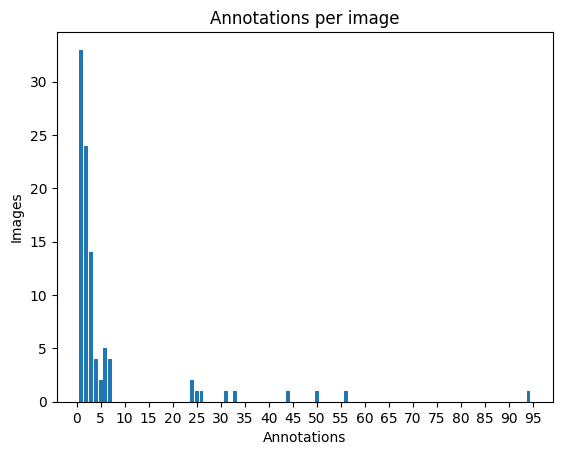
\includegraphics[width=0.8\textwidth]{chapter3/annotations_per_img.png}
    \caption{Overview of the annotations per image in the shell dataset.}
    \label{fig:annotations_per_img}
\end{figure}

\begin{table}[H]
    \centering
    \captionsetup{justification=centering}
    \begin{tabular}{|c|c|c|}
    \hline
    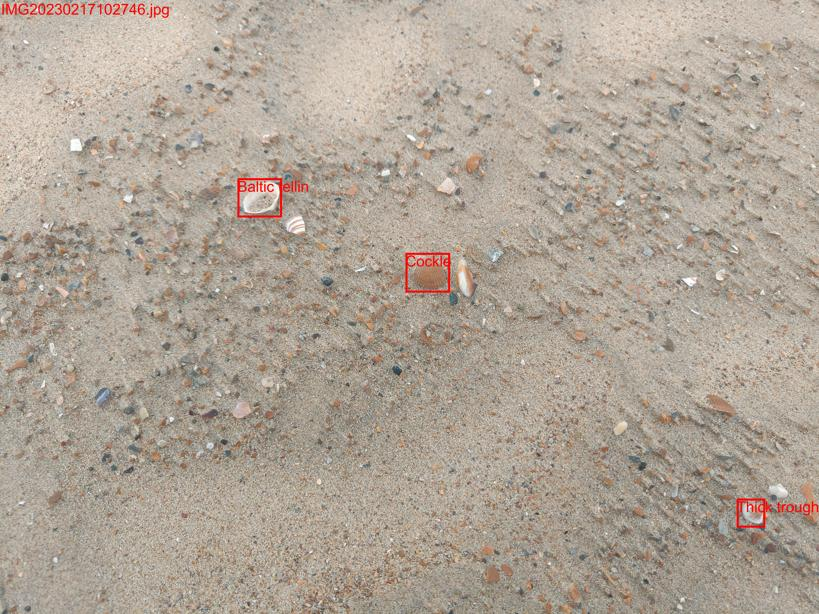
\includegraphics[width=0.3\textwidth]{chapter3/shell_examples/1.jpg} & 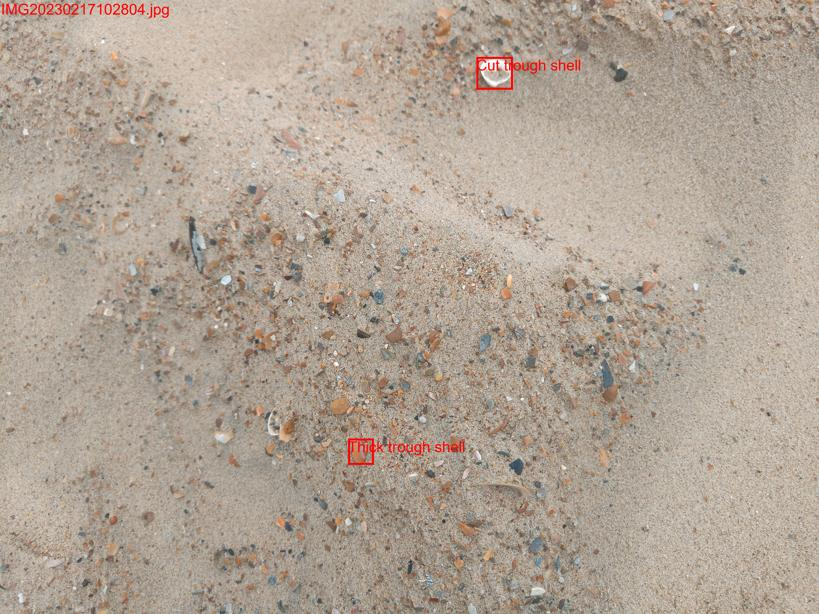
\includegraphics[width=0.3\textwidth]{chapter3/shell_examples/2.jpg} & 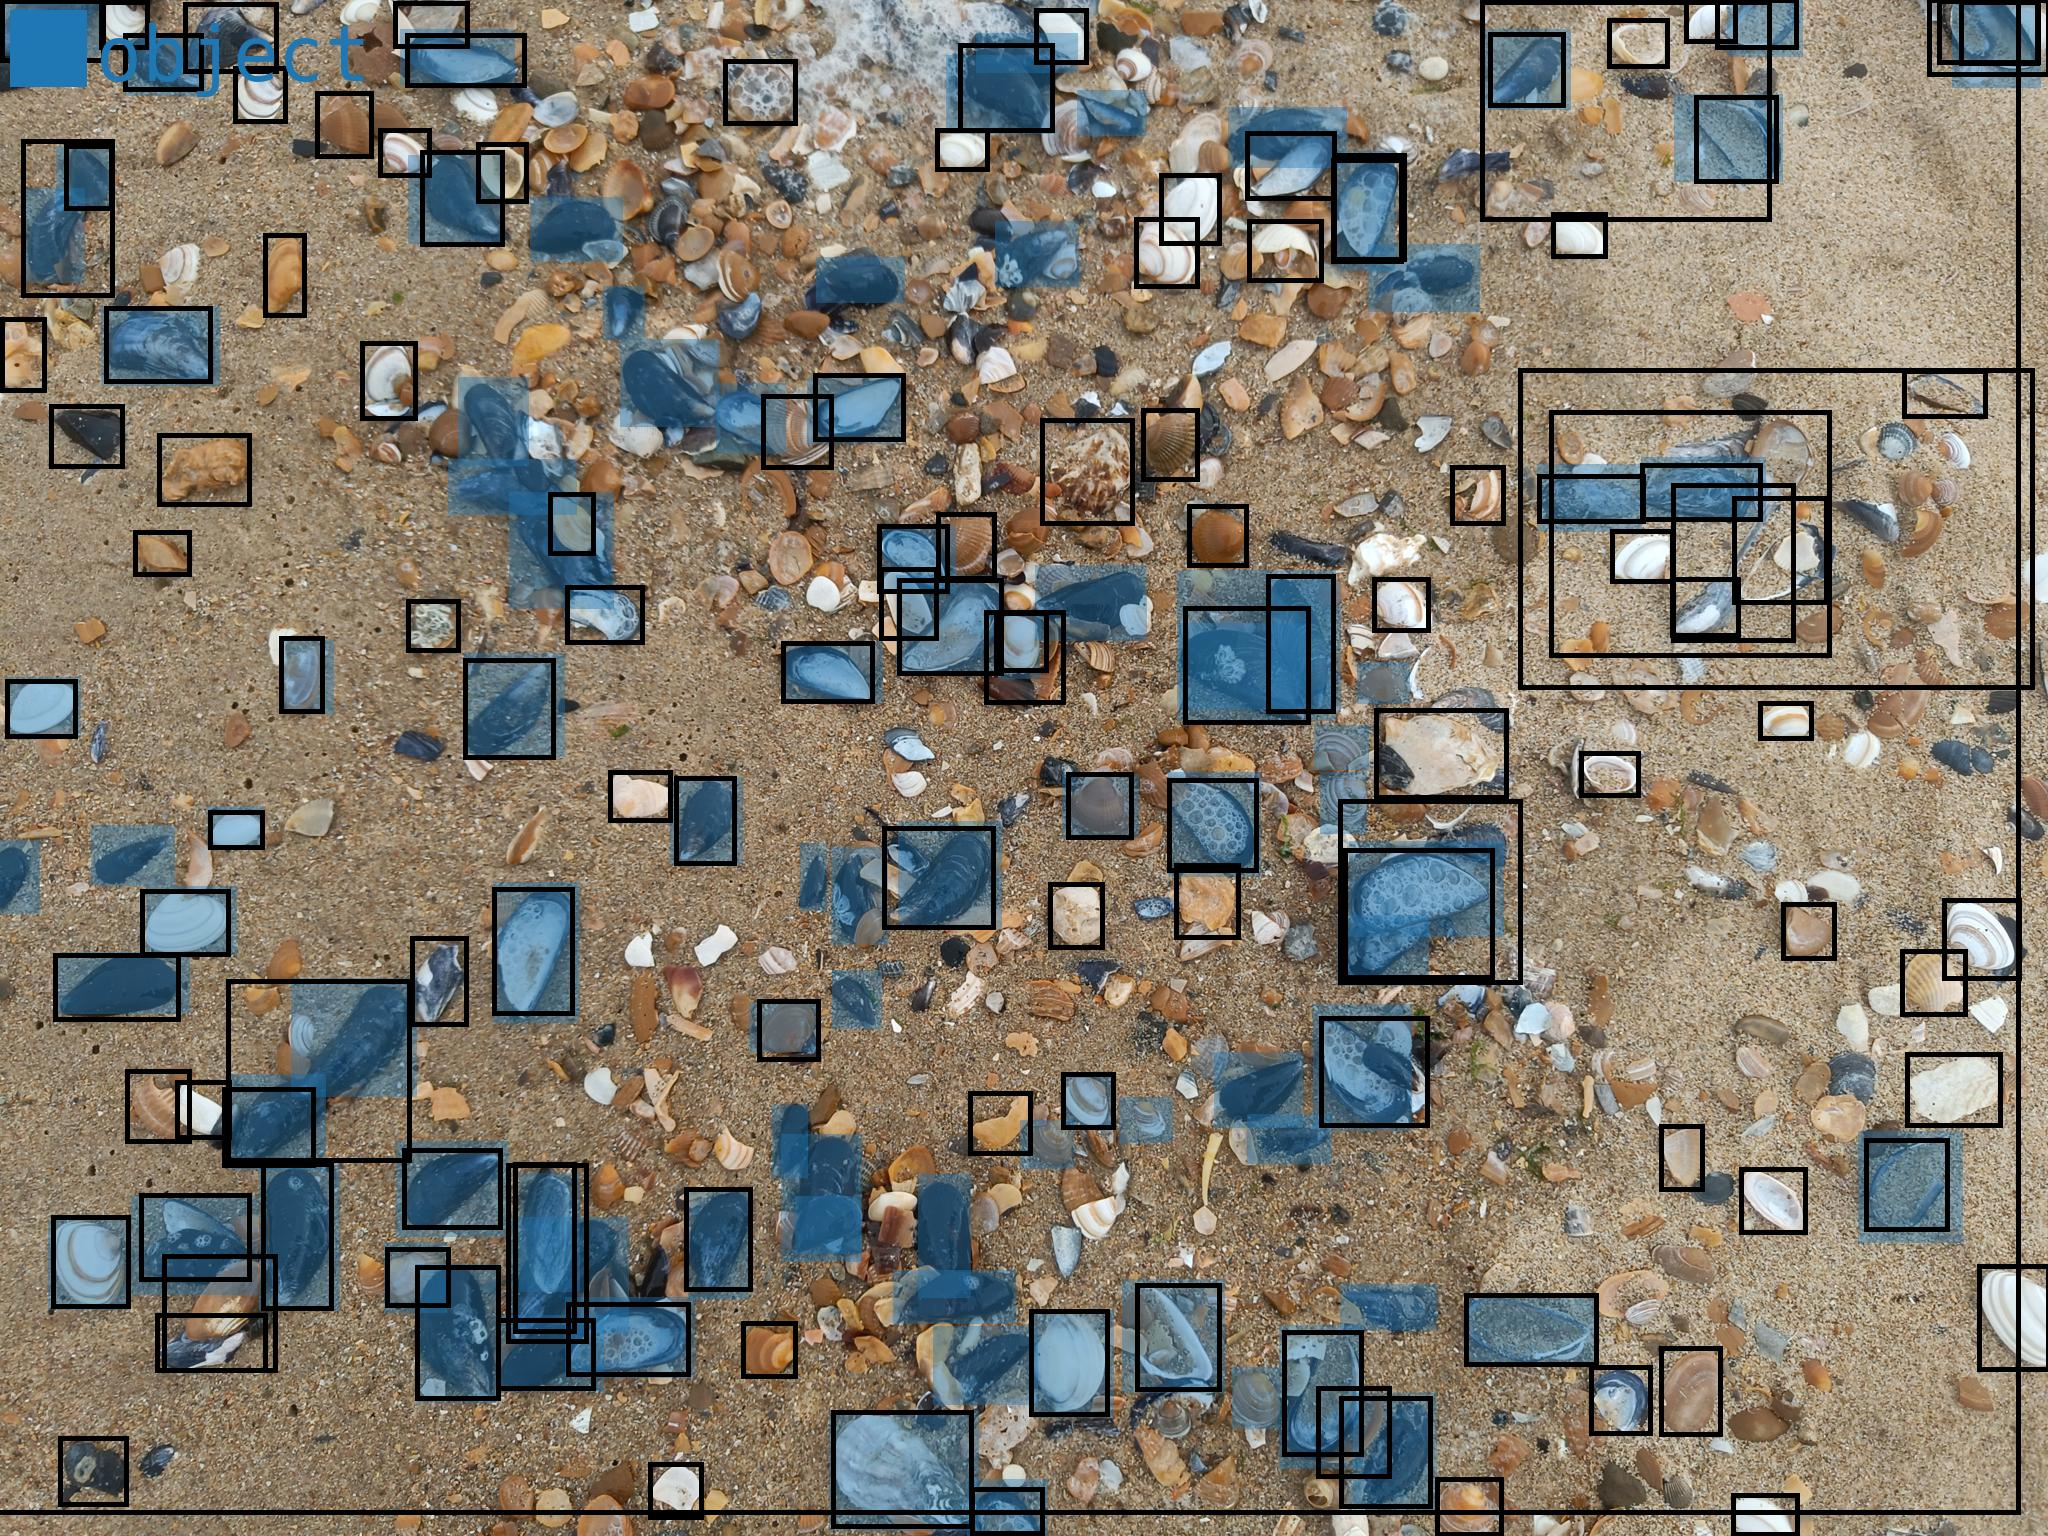
\includegraphics[width=0.3\textwidth]{chapter3/shell_examples/3.jpg} \\ \hline
    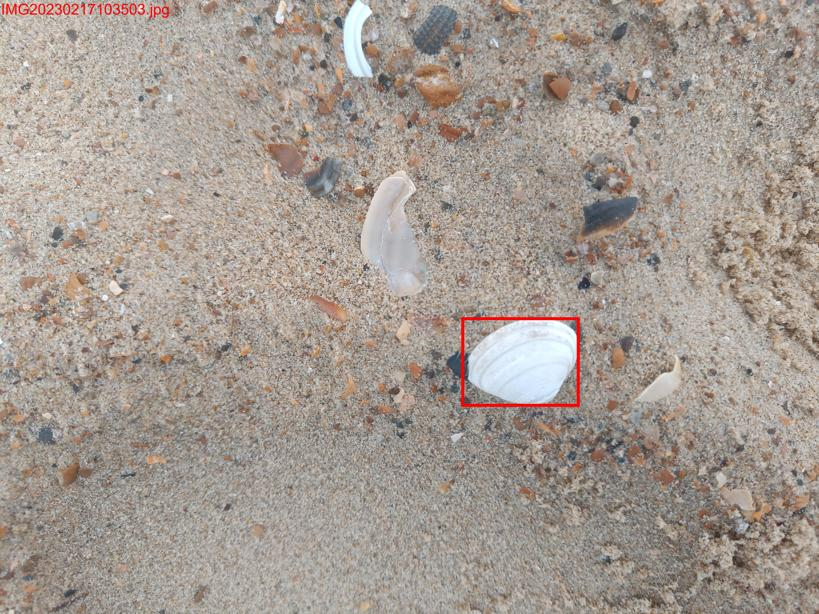
\includegraphics[width=0.3\textwidth]{chapter3/shell_examples/4.jpg} & 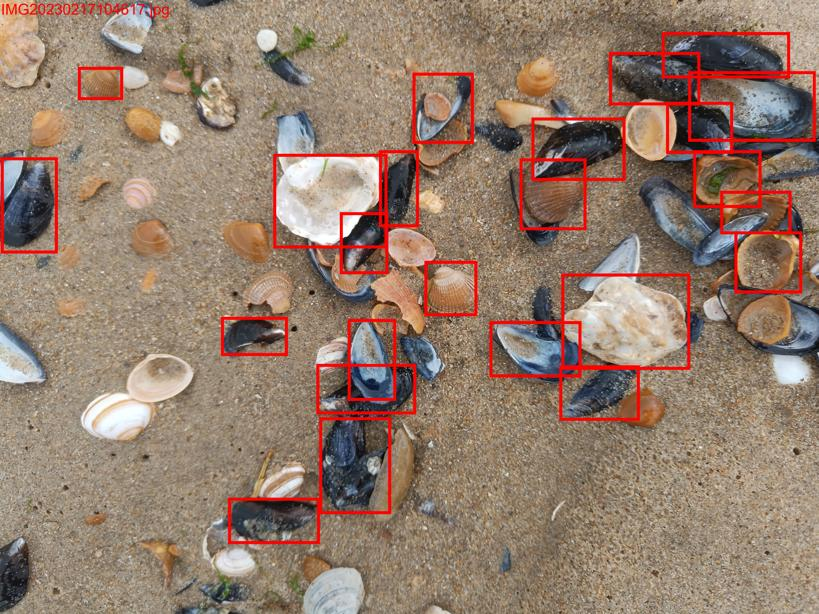
\includegraphics[width=0.3\textwidth]{chapter3/shell_examples/5.jpg} & 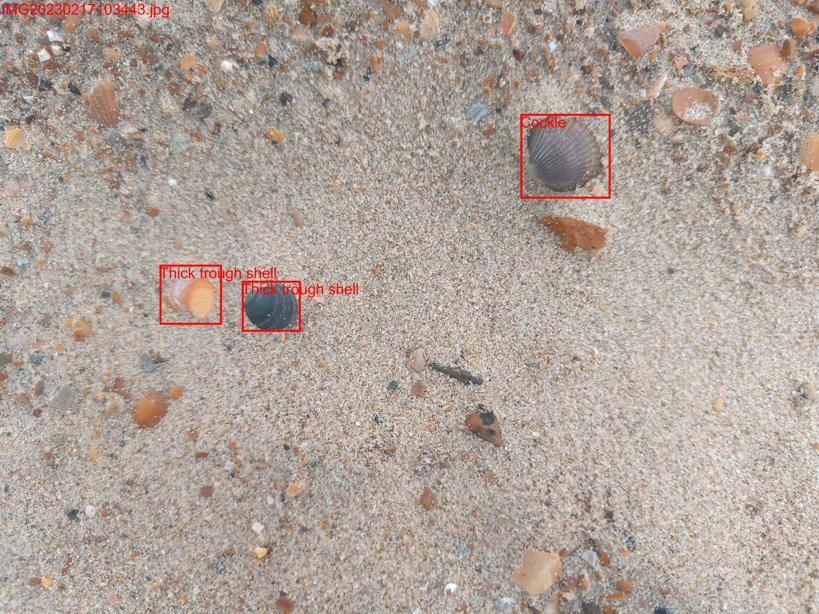
\includegraphics[width=0.3\textwidth]{chapter3/shell_examples/6.jpg} \\ \hline
    \rotatebox{90}{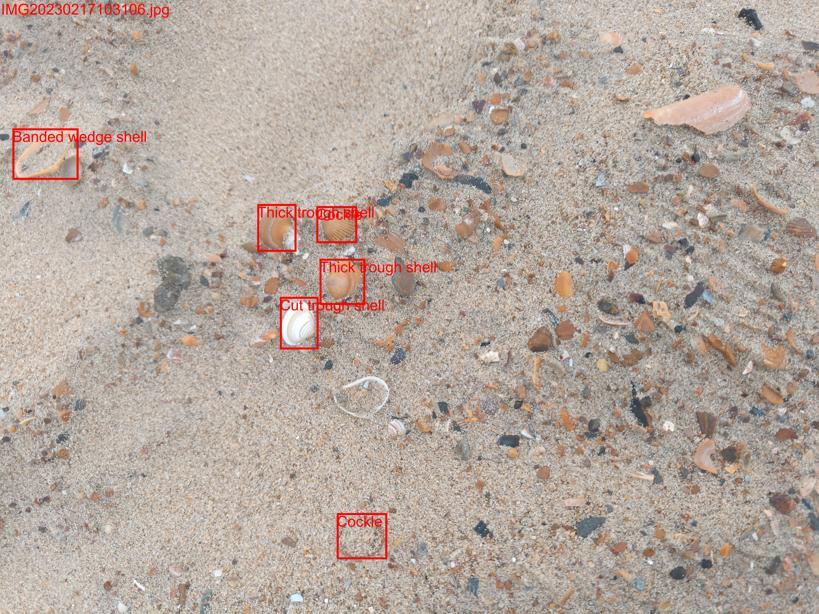
\includegraphics[height=0.3\textwidth]{chapter3/shell_examples/7.jpg}} & \rotatebox{90}{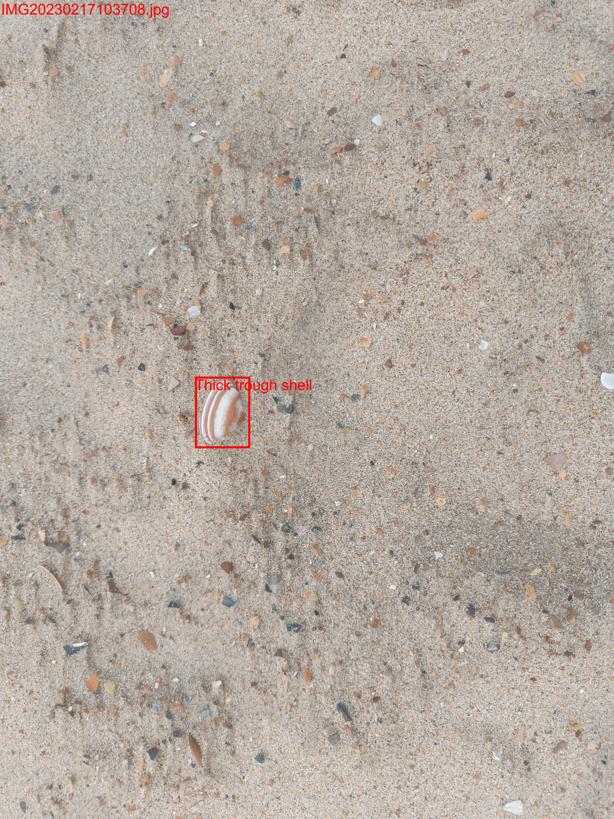
\includegraphics[height=0.3\textwidth]{chapter3/shell_examples/8.jpg}} & \rotatebox{90}{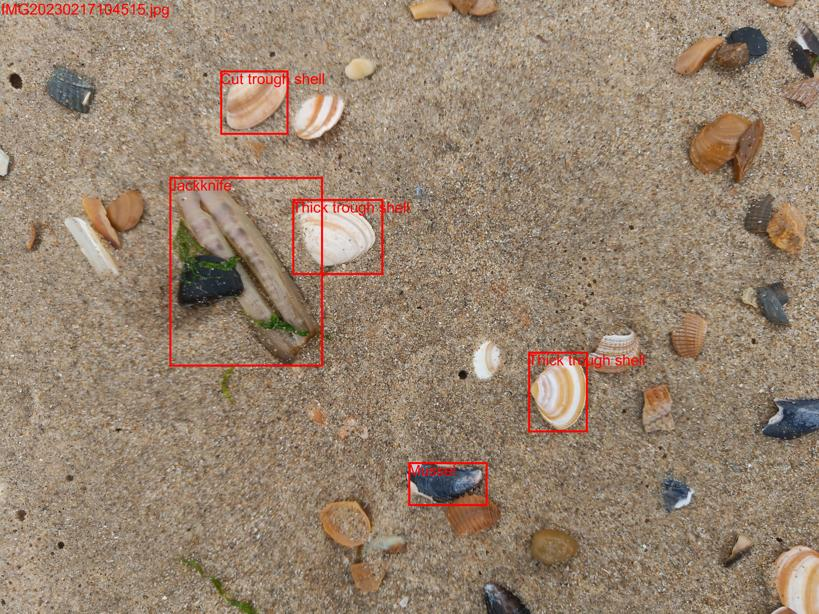
\includegraphics[height=0.3\textwidth]{chapter3/shell_examples/9.jpg}} \\ \hline
    \end{tabular}
    \caption{Examples of images in the shell dataset.}
    \label{tab:shell_examples}
\end{table}

\section{Baseline}
In this section, we establish a baseline for the shell dataset. For this, we will study the performance of OWL-ViT with image-based one-shot detection. 

\subsection{Model}
For the baseline, we will use the OWL-ViT model. A short description is made in section \ref*{sec:2_owlvit}. At inference time embeddings are extracted from the image using the ViT encoder. These object image embeddings are then compared to the query (text or image) embeddings as shown in figure \ref{fig:2_owl-vitr} to obtain a similarity score. The model exists in different flavors, with different backbones and different patch sizes. Hardware limitations limit us to the smallest ViT-B/32 model.

The model is implemented using the Scenic library \citep{scenic}. 
It is also included in the transformers library, which offers an abstraction layer for running the model. Running the model is done by loading the processor and model, using the processor on the query images and test image to obtain the inputs for the model and then running the model.

\subsection{Inference}
Setting up for inference follows the following steps:
\begin{enumerate}
    \item Load the model and processor.
        \begin{itemize}
            \item The model and processor are readily available from the transformers library.
        \end{itemize}
    \item Load the images and annotations.
        \begin{itemize}
            \item The images are Pascal VOC annotated, they are loaded into a class that offers the needed functionality.
        \end{itemize}
    \item Extract a query image for each class from the annotated images.
        \begin{itemize}
            \item The query images are extracted from the first image that contains an annotation of that class.
            \item Optionally the images can be shuffled to obtain a different query image for each class.
            \item The image from which the query image was taken is then removed from the test set. 
        \end{itemize}
    \item (Optional) Remove the background from the query images.
        \begin{itemize}
            \item The background is removed using the rembg library, which uses a neural network (u2net) to remove the background.
        \end{itemize}
\end{enumerate}
Inference is then done by doing image-guided detection with all the query images on each of the test images sequentially due to hardware limitations. 

\subsection{Processing}
To process the results, we can do the following operations [with these parameters]:
\begin{itemize}
    \item NMS [True, False]
    \begin{itemize}
        \item IoU threshold [0.1, 0.2, ..., 0.9]
    \end{itemize}
    \item Apply confidence threshold [0.01, 0.02, ..., 0.99]
    \item Filter excessively large boxes [True, False]
    \begin{itemize}
        \item We found that the model produces many excessively large boxes, which are filtered out if this parameter is set. 
    \end{itemize}
\end{itemize}
To find the optimal parameters, we create a grid of all possible combinations of these parameters. For each of the 4444 combinations, we process the model outputs. This returns the number of correct detections, correct bounding boxes, wrong detections and missed detections for each combination.

To evaluate the results we use the metrics described in section \ref{sec:2_metrics}. Correct detections are the true positives, wrong detections and correct bounding boxes are the false positives and missed detections are the false negatives. We could calculate the metrics for getting the bounding box correct by taking the correct detections and the correct bounding boxes as true positives and only the wrong detections as false positives, but that is not relevant to our use case.

By calculating the metrics for each combination of parameters, we can discover the impact of each parameter on the performance of the model. 

As seen in figure \ref{fig:3_nms}, enabling NMS will in most cases remove more true positives than false positives, and thus decrease the performance of the model. Some outliers do however show that NMS can improve the precision of the model in some cases.

% nms precision and recall
\begin{figure}[h]
    \begin{adjustwidth}{-1in}{-1in}
        \centering
        \begin{subfigure}[b]{0.45\paperwidth}
            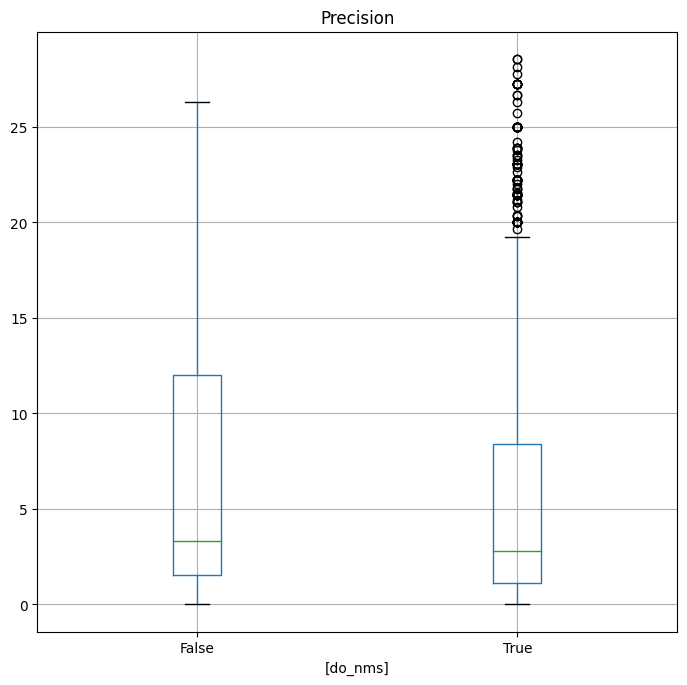
\includegraphics[width=\textwidth]{chapter3/owl-vit/nms_precision.png}
            \caption{Precision}
            \label{fig:3_nms_precision}
        \end{subfigure}
        \begin{subfigure}[b]{0.45\paperwidth}
            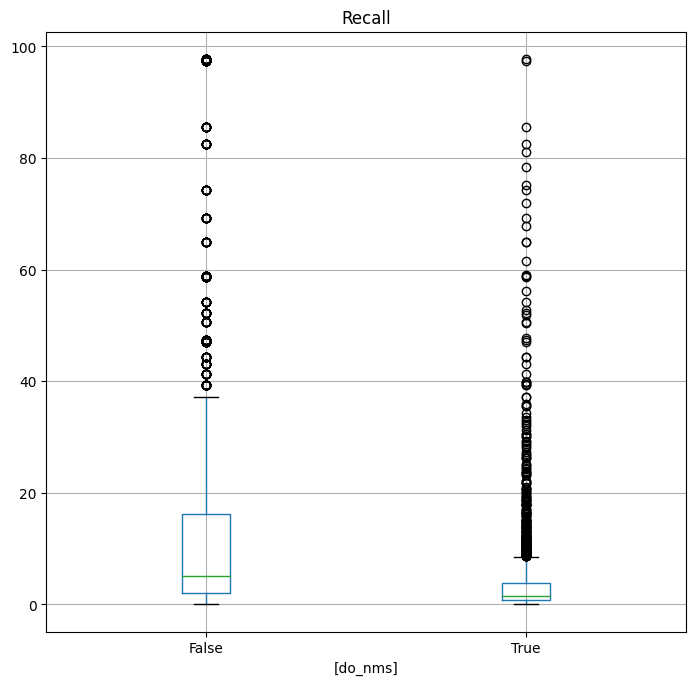
\includegraphics[width=\textwidth]{chapter3/owl-vit/nms_recall.png}
            \caption{Recall}
            \label{fig:3_nms_recall}
        \end{subfigure}
    \end{adjustwidth}
    \caption{Precision and recall for different IoU thresholds.}
    \label{fig:3_nms}
\end{figure}

As seen in figure \ref{fig:3_confidence}, raising the confidence threshold will predicably reduce the recall while increasing the precision. The recall drops sharply, however, dropping to 20\% at a confidence threshold of 0.2. Though increasing the confidence threshold does increase the precision as it eliminates more false than true positives, the recall drops so sharply that the overall performance of the model is reduced beyond the realm of usefulness.

% confidence precision and recall
\begin{figure}[h]
    \centering
    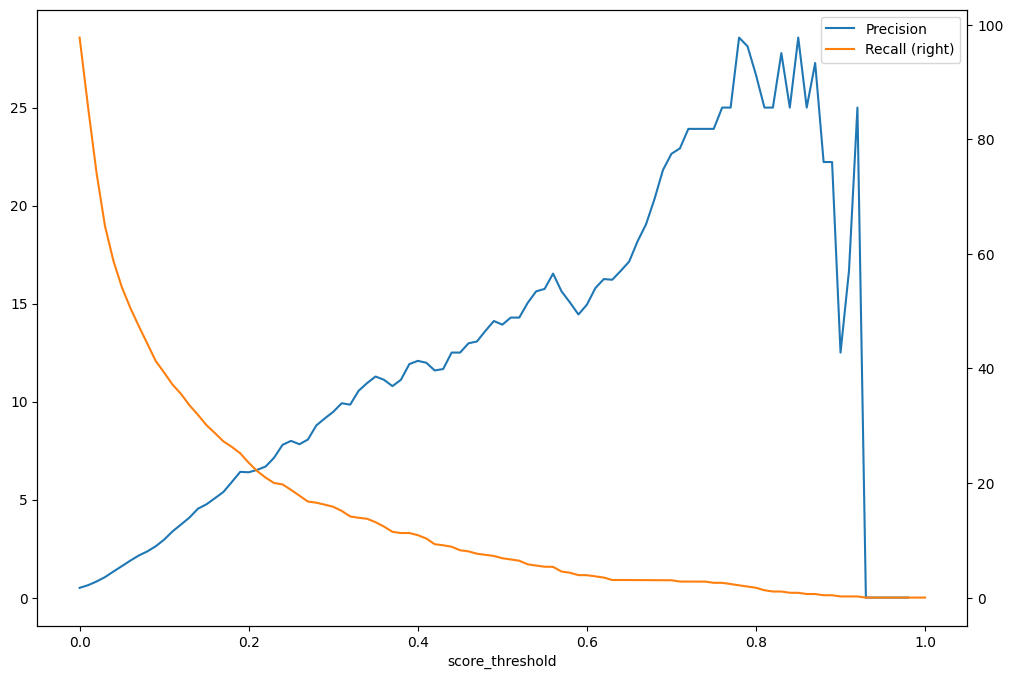
\includegraphics[width=\textwidth]{chapter3/owl-vit/confidence.png}
    \caption{Max precision and recall for different confidence thresholds.}
    \label{fig:3_confidence}
\end{figure}

As seen in figure \ref{fig:3_iou_mean_max}, the IoU threshold has a large impact on the recall of the model. As fewer bounding boxes are eliminated, the recall increases with a higher threshold. The precision takes little to impact from varying the IoU threshold, making a good case for disabling NMS altogether.

% iou mean and max precision and recall
\begin{figure}[h]
    \begin{adjustwidth}{-1in}{-1in}
        \centering
        \begin{subfigure}[b]{0.45\paperwidth}
            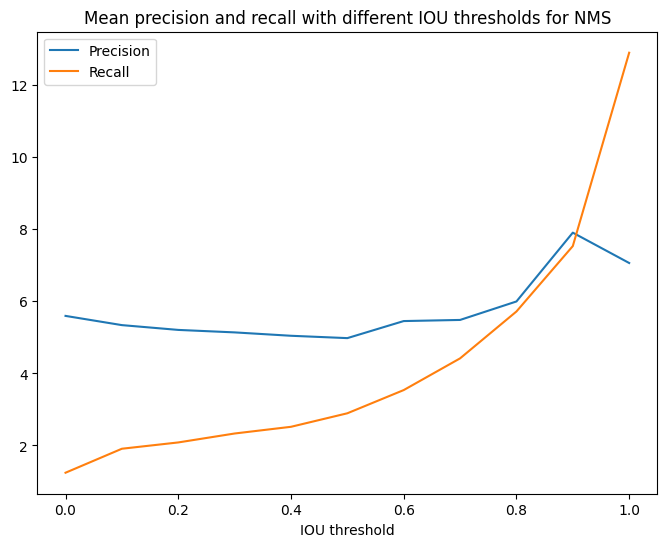
\includegraphics[width=\textwidth]{chapter3/owl-vit/iou_mean.png}
            \caption{Mean precision}
            \label{fig:3_iou_mean_precision}
        \end{subfigure}
        \begin{subfigure}[b]{0.45\paperwidth}
            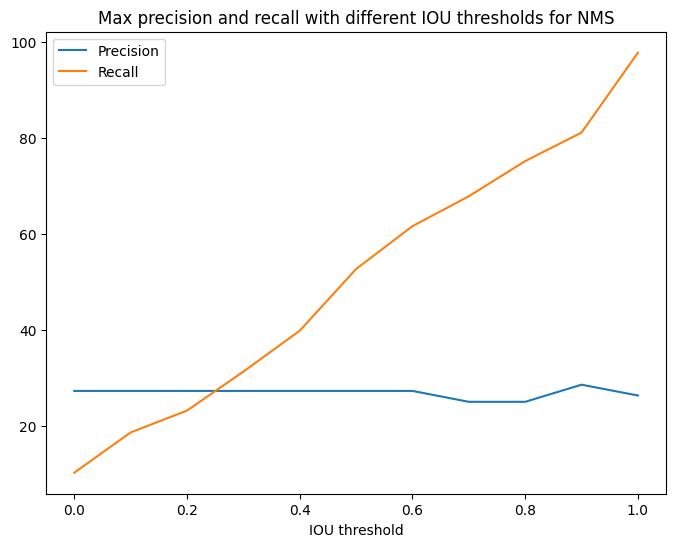
\includegraphics[width=\textwidth]{chapter3/owl-vit/iou_max.png}
            \caption{Mean recall}
            \label{fig:3_iou_mean_recall}
        \end{subfigure}
    \end{adjustwidth}
    \caption{Mean and max precision and recall for different IoU thresholds.}
    \label{fig:3_iou_mean_max}
\end{figure}

Looking at figure \ref{fig:3_filter}, we see that filtering excessively large boxes improves precision by a large margin, with little to no impact on the recall. The model produces many excessively large boxes, which are filtered out if this parameter is set. The caveat is that this is technically cheating, as in the current implementation the solution is being used for this filtering. This could be improved upon by using a different approach to find appropriate measurements for filtering excessively large boxes.

% filter precision and recall
\begin{figure}[h]
    \begin{adjustwidth}{-1in}{-1in}
        \centering
        \begin{subfigure}[b]{0.45\paperwidth}
            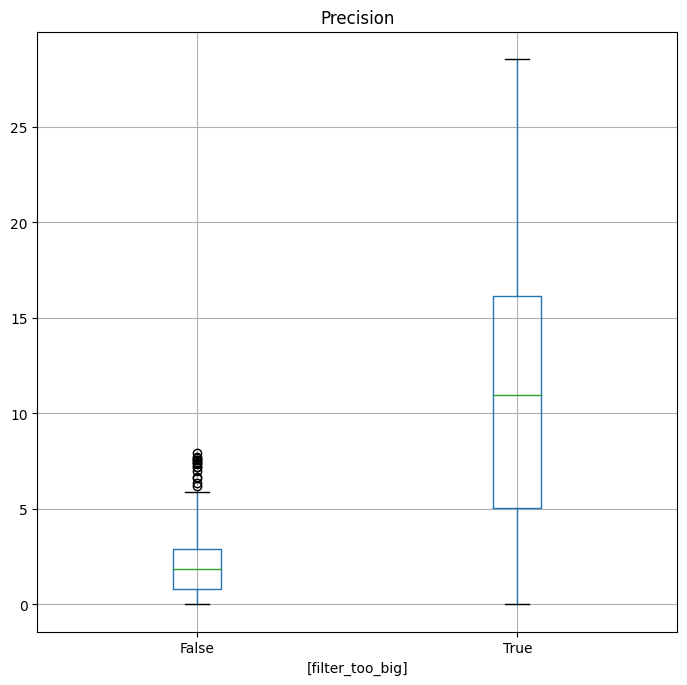
\includegraphics[width=\textwidth]{chapter3/owl-vit/filter_precision.png}
            \caption{Precision}
            \label{fig:3_filter_precision}
        \end{subfigure}
        \begin{subfigure}[b]{0.45\paperwidth}
            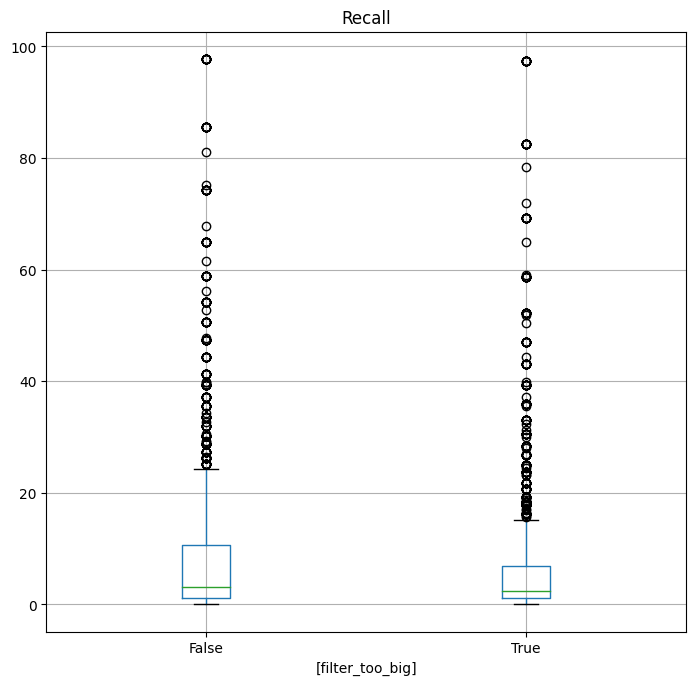
\includegraphics[width=\textwidth]{chapter3/owl-vit/filter_recall.png}
            \caption{Recall}
            \label{fig:3_filter_recall}
        \end{subfigure}
    \end{adjustwidth}
    \caption{Precision and recall for filtering excessively large boxes.}
    \label{fig:3_filter}
\end{figure}

\subsection{Results}
